\documentclass[12pt]{amsart}
\usepackage[margin=1in]{geometry}       % page margins
\usepackage{setspace}                   % line spacing
\usepackage{hyperref}                   % clickable links & cross-refs
\usepackage{booktabs}                   % professional tables
\usepackage{natbib}                     % citations (author-year)
\usepackage{lipsum}                     % placeholder text — REMOVE when done
\usepackage{graphicx, physics}
\usepackage{fancyhdr}
\usepackage{ragged2e}
\usepackage{amsmath, amsthm, amssymb}
\usepackage{tikz}
\usepackage{float}
\usetikzlibrary{shapes.geometric, backgrounds, calc, arrows.meta, arrows, positioning, fit}
\newcommand{\xsfit}{\scriptsize}

\hypersetup{
    colorlinks = true,
    linkcolor  = blue,
    citecolor  = blue,
    urlcolor   = blue
}
\doublespacing

% ============================================================
%  TITLE MATTER
% ============================================================

\title[]{%
    \large{\textbf{}}\\[0.2em]
    \small {Designing a Quantum Inspired Optical Accelerator}%
}

% ── Authors ─────────────────────────────────────────────────
% Each author gets their own \author, \address, \email block.
% amsart renders these visibly below the title.
% Use \and between authors if listing on one \author line,
% or give each their own block as shown here.

\author{Zoeb Izzi}
\address{Quantum Physics \& Optics Lab, Thomas Jefferson High School for Science \& Technology, Alexandria, VA, USA}
\email{2027ZIzzi@tjhsst.edu}

% ── Corresponding author footnote ───────────────────────────
% \thanks attaches a footnote to whichever \author it follows.
% Move it to the right author block above, e.g.:
%   \author{First Author\thanks{Corresponding author.}}
\thanks{%
}
\date{\today}
\begin{document}
    \begin{abstract}
        This paper presents a design for an optical quantum emulator that uses coherent, classical lasers to emulate certain quantum computations. It uses NPBS to generate beams of photons that can (with caution) be treated as qubits and uses gates mounted on motorized platforms to manipulate them, with unary gates being represented by variations on the angle of half-wave plates and quarter-wave plates and binary/multinary gates being represented by a module design that uses a Polarizing Beam Splitter (PBS) to split a target beam, applying the appropriate transformations to one of the beams, and using an AOM to postselect the correct outcomes based on the state of the control beam(s). The end result is that correlated pairs are generated, where an individual sub-beam of control and target will have correctly correlated (simulating entangled) states; either the control will be horizontally polarized and the target will be unchanged, or the control will be vertically polarized and the target will be rotated (in the case of CNOT; alternate controlled gates will be adjusted as needed). The design is easily scalable because of its motorized design and, because it uses classical lasers rather than single photon generators, has the potential to be far cheaper than most current quantum computers.  
    \end{abstract}
    \maketitle
    \newpage
    \tableofcontents
    \newpage


    \section{The Design}
    \label{sec:Design 2}
    This design uses coherent lasers to generate a large number of photons that can be manipulated to emulate quantum states. By using a continuous laser source, we can create a high-intensity beam that can be split and routed through various optical elements to perform quantum operations. This approach allows for the generation of many qubits simultaneously, making it more scalable than the SPDC-based design. Further, lasers are far cheaper than single photon generators, which makes this design far cheaper than the first. Note that the setups (e.g. the single-qubit rotation gates, the pipeline of operation, and the motorization of the gate systems) are the same as in the first design.

    \subsection{Qubit Generation}
    \label{subsec:Qubit Generation}
    
    Using the high powered laser source, we use a variety of Non-Polarizing Beam Splitters (NPBS) to split the laser beam into multiple paths, each representing a qubit. The polarization of the laser light can be manipulated using wave plates to encode quantum information. Since NPBS does not affect polarization of light, we can use it to generate the "qubits" as needed. The initial beam setup, without loss of generality, can be modeled as follows (using additional NPBS and mirrors to create a larger system as needed):

    \begin{figure}[hbtp]
        \centering
        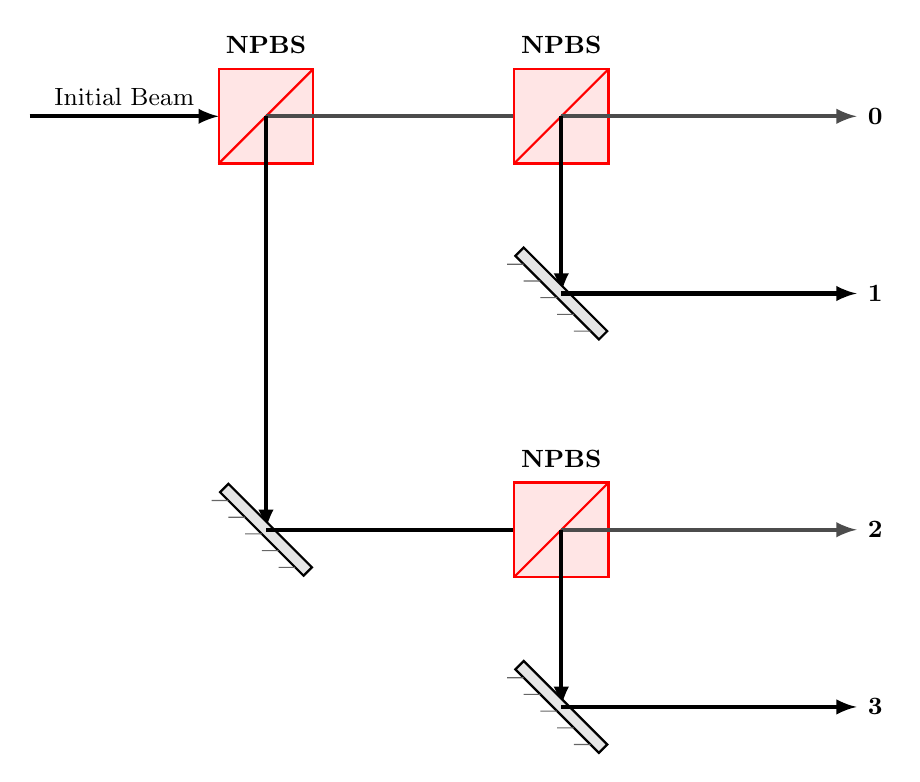
\begin{tikzpicture}[
    scale=1.5,
    ray/.style={line width=1.5pt, black, -latex},
    trans_ray/.style={line width=1.5pt, black!70, -latex},
    ref_ray/.style={line width=1.5pt, black, -latex},
    component/.style={draw=red, fill=red!10, thick}, % NPBS Cubes: Red outline, light red fill
    mirror/.style={draw=black, fill=black!10, thick}   % Mirrors: Black/gray
]

    % --- STAGE 1 COORDINATES ---
    \coordinate (LaserStart) at (0,0);
    \coordinate (PBS1) at (2,0);
    \coordinate (M1) at (2,-3.5);

    % --- STAGE 2 COORDINATES ---
    \coordinate (PBS2) at (4.5,0);
    \coordinate (M2) at (4.5,-1.5);
    
    \coordinate (PBS3) at (4.5,-3.5);
    \coordinate (M3) at (4.5,-5.0);

    % --- OUTPUT TERMINALS ---
    \coordinate (Out1) at (7,0);
    \coordinate (Out2) at (7,-1.5);
    \coordinate (Out3) at (7,-3.5);
    \coordinate (Out4) at (7,-5.0);

    % ==========================================
    % STAGE 1: FIRST SPLIT (1 -> 2 Beams)
    % ==========================================

    % Draw Input Laser Beam
    \draw[ray] (LaserStart) -- ($(PBS1) - (0.4,0)$) node[midway, above, black, font=\small] {Initial Beam};
    \draw[ray] ($(PBS1) - (0.4,0)$) -- (PBS1);

    % Draw NPBS 1
    \draw[component] ($(PBS1) - (0.4,0.4)$) rectangle ($(PBS1) + (0.4,0.4)$);
    \draw[red, thick] ($(PBS1) - (0.4,0.4)$) -- ($(PBS1) + (0.4,0.4)$);
    \node[black, font=\small\bfseries] at ($(PBS1) + (0,0.6)$) {NPBS};

    % Top Path (Straight to Stage 2)
    \draw[trans_ray] (PBS1) -- (PBS2);

    % Bottom Path (Down to Mirror 1)
    \draw[ref_ray] (PBS1) -- (M1);

    % Mirror 1
    \begin{scope}[shift={(M1)}]
        \draw[mirror, rotate=-45] (-0.5,-0.05) rectangle (0.5,0.05);
        \foreach \x in {-0.4,-0.2,0,0.2,0.4} {
            \draw[black!60, thin, rotate=-45] (\x, -0.05) -- (\x-0.1, -0.15);
        }
    \end{scope}

    % Bottom Path (Redirected to Stage 2)
    \draw[ref_ray] (M1) -- (PBS3);


    % ==========================================
    % STAGE 2: SECOND SPLIT (2 -> 4 Beams)
    % ==========================================

    % --- UPPER REPEATER TREE ---
    % Draw NPBS 2
    \draw[component] ($(PBS2) - (0.4,0.4)$) rectangle ($(PBS2) + (0.4,0.4)$);
    \draw[red, thick] ($(PBS2) - (0.4,0.4)$) -- ($(PBS2) + (0.4,0.4)$);
    \node[black, font=\small\bfseries] at ($(PBS2) + (0,0.6)$) {NPBS};

    % Beam 0 Out (Straight)
    \draw[trans_ray] (PBS2) -- (Out1) node[right, black, font=\small\bfseries] {0};

    % Beam 1 Down to Mirror 2
    \draw[ref_ray] (PBS2) -- (M2);

    % Mirror 2
    \begin{scope}[shift={(M2)}]
        \draw[mirror, rotate=-45] (-0.5,-0.05) rectangle (0.5,0.05);
        \foreach \x in {-0.4,-0.2,0,0.2,0.4} {
            \draw[black!60, thin, rotate=-45] (\x, -0.05) -- (\x-0.1, -0.15);
        }
    \end{scope}

    % Beam 1 Out (Redirected)
    \draw[ref_ray] (M2) -- (Out2) node[right, black, font=\small\bfseries] {1};


    % --- LOWER REPEATER TREE ---
    % Draw NPBS 3
    \draw[component] ($(PBS3) - (0.4,0.4)$) rectangle ($(PBS3) + (0.4,0.4)$);
    \draw[red, thick] ($(PBS3) - (0.4,0.4)$) -- ($(PBS3) + (0.4,0.4)$);
    \node[black, font=\small\bfseries] at ($(PBS3) + (0,0.6)$) {NPBS};

    % Beam 2 Out (Straight)
    \draw[trans_ray] (PBS3) -- (Out3) node[right, black, font=\small\bfseries] {2};

    % Beam 3 Down to Mirror 3
    \draw[ref_ray] (PBS3) -- (M3);

    % Mirror 3
    \begin{scope}[shift={(M3)}]
        \draw[mirror, rotate=-45] (-0.5,-0.05) rectangle (0.5,0.05);
        \foreach \x in {-0.4,-0.2,0,0.2,0.4} {
            \draw[black!60, thin, rotate=-45] (\x, -0.05) -- (\x-0.1, -0.15);
        }
    \end{scope}

    % Beam 3 Out (Redirected)
    \draw[ref_ray] (M3) -- (Out4) node[right, black, font=\small\bfseries] {3};

\end{tikzpicture}
    \end{figure}

    \subsection{Optical Gate Manipulation}
    \label{subsec:Optical Gate Manipulation}
    All of the unary gates (gates that involve only 1 qubit) are standard: X gate represented by a HWP-0, Z-gate represented by HWP-45, Hadamard by HWP-22.5, Y gate represented by QWP-45 and HWP-45. However, this design uses temporal variation to simulate the CNOT effect. By introducing a randomization by which the control qubit and target qubit are outputted probabilistically depending on the relative probabilities of the control qubit, allowing both coherent beams to exist and picking only one to go through, we preserve the "entanglement" effect of the CNOT gate (simulated here by not allowing the target qubit without the X gate to be outputted if the control qubit ouputs $\ket{V}$, and vice versa). This design is also more physically intensive, as it requires a lot of mirrors and beam splitters to ensure that the qubits are outputted in the correct order. We represent it as follows:

\begin{figure}[htbp]
    \centering
    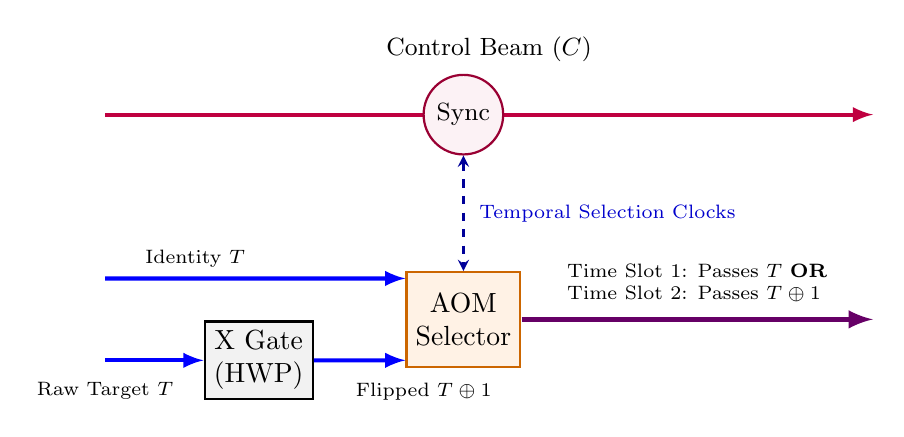
\begin{tikzpicture}[
        scale=1.3,
        control_ray/.style={line width=1.5pt, purple, -latex},
        target_ray/.style={line width=1.5pt, blue, -latex},
        combined_ray/.style={line width=2pt, violet!80!black, -latex},
        component/.style={draw=black, fill=gray!10, thick, minimum width=1.2cm, minimum height=0.8cm, align=center},
        aom/.style={draw=orange!80!black, fill=orange!10, thick, minimum width=1.4cm, minimum height=1.2cm, align=center}
    ]

        % --- Control Line (Unchanged) ---
        \coordinate (C_In) at (0, 1.5);
        \coordinate (C_Out) at (7.5, 1.5);
        \draw[control_ray] (C_In) -- (C_Out) node[midway, above=15pt, black, font=\small] {Control Beam ($C$)};
        
        % Timing Synchronizer Hub Node
        \node[draw=purple!80!black, fill=purple!5, thick, circle, inner sep=3pt] (AOM_Ctrl) at (3.5, 1.5) {\small Sync};

        % --- Target Module (Shifted down by 0.5) ---
        % AOM Selector moved from (3.5, 0) to (3.5, -0.5)
        \node[aom] (AOM_Selector) at (3.5, -0.5) {AOM\\Selector};
        \node[component] (X_Gate) at (1.5, -0.9) {X Gate\\(HWP)};
        
        \coordinate (T_In_Raw) at (0, -0.1);
        \coordinate (T_In_Flip) at (0, -0.9);
        \coordinate (T_Out) at (7.5, -0.5);

        % Drawing the Input paths into the AOM
        \draw[target_ray] (T_In_Raw) -- ($(AOM_Selector.west) + (0, 0.4)$) 
            node[pos=0.3, above, black, font=\scriptsize] {Identity $T$};
            
        \draw[target_ray] (T_In_Flip) -- (X_Gate.west) 
            node[pos=0, below=4pt, black, font=\scriptsize] {Raw Target $T$};
        \draw[target_ray] (X_Gate.east) -- ($(AOM_Selector.west) + (0, -0.4)$) 
            node[pos=1.2, below=4pt, black, font=\scriptsize] {Flipped $T \oplus 1$};

        % --- Output Ray and Text ---
        \draw[combined_ray] (AOM_Selector.east) -- (T_Out) 
            node[pos=0.5, above=2pt, black, font=\scriptsize, align=left] {Time Slot 1: Passes $T$ \textbf{OR} \\ Time Slot 2: Passes $T \oplus 1$};

        % Extended Software Sync Signal (Longer vertical gap)
        \draw[dashed, thick, <->, >=stealth, blue!60!black] (AOM_Ctrl.south) -- (AOM_Selector.north) 
            node[midway, right=2pt, font=\scriptsize, text=blue!80!black] {Temporal Selection Clocks};

\end{tikzpicture}
\caption{Temporal selection routing featuring expanded vertical gap spacing between the control path and the modulated AOM architecture.}
\label{fig:aom_selector_shifted}
\end{figure}
    Over time, in a sufficiently large time interval (assuming the control qubit is in a superposition of $\ket{H}$ and $\ket{V}$), the target qubit will be flipped with probability $p$ and passed unchanged with probability $1-p$, where $p$ is the probability of the control qubit being in the $\ket{V}$ state. This effectively simulates the CNOT operation, as the target qubit's state is conditionally modified based on the control qubit's state.

    To confirm, let's assume the control qubit is in a superposition state $\ket{\psi_C} = \alpha\ket{H} + \beta\ket{V}$, and the target qubit is in state $\ket{\psi_T} = \gamma \ket{H} + \delta \ket{V}$. The target qubit is initially in state $\ket{\psi_T}$. After the X gate is applied, we have 2 targets, one of which is $\ket{\psi_T} = \gamma \ket{H} + \delta \ket{V}$ and the other of which is $\ket{\psi_T'} = \delta \ket{H} + \gamma \ket{V}$. The AOM then selects one of these two targets based on the control qubit's state. If the control qubit is in state $\ket{H}$, the AOM will select $\ket{\psi_T}$, and if the control qubit is in state $\ket{V}$, the AOM will select $\ket{\psi_T'}$. Over time, this results in the target qubit being flipped with probability $|\beta|^2$ and passed unchanged with probability $|\alpha|^2$, effectively simulating the CNOT operation. Further, we can preserve the phase by emitting the polarization in the correct direction and with the correct attached phase from the CNOT emitter. Since these are coherent light beams, we need only ensure that the timing is synchronized, which is what the AOM is specifically useful for. Further, the detectors can simply be those that detect if light is being shined in (combined with a PBS, this will tell us what the polarization of the light is). 

    Further, the detector setup is as follows for the CNOT detector, since that must be more in depth to copy the phase outputs as well:
\begin{figure}[htbp]
\centering

    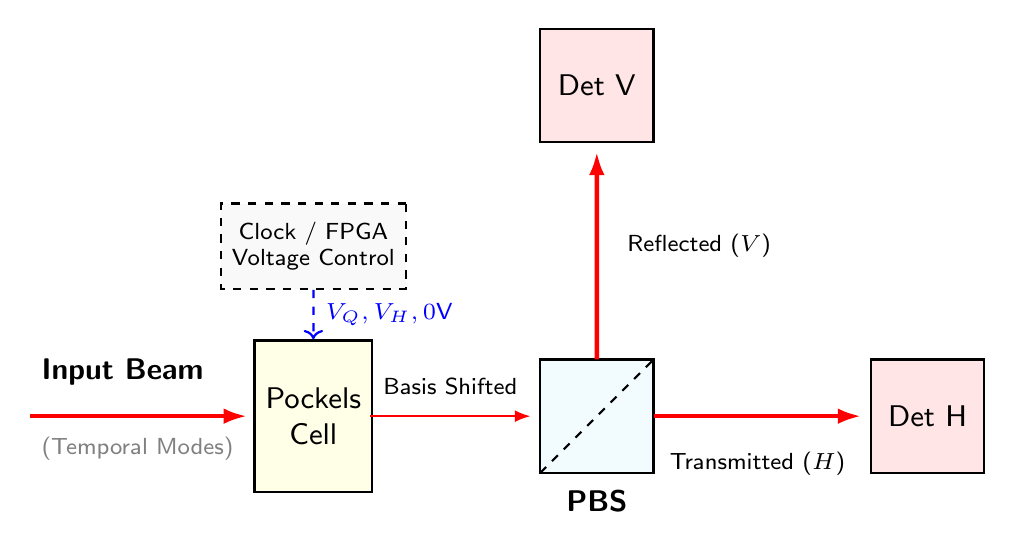
\begin{tikzpicture}[
    scale=1.2, 
    every node/.style={transform shape},
    component/.style={draw, thick, fill=yellow!10, minimum width=1.0cm, minimum height=1.6cm, align=center, font=\small\sffamily},
    detector/.style={draw, thick, fill=red!10, minimum width=1.2cm, minimum height=1.2cm, font=\small\sffamily, align=center}
]

    % --- Input Beam & Label ---
    \draw[-{Latex[length=3mm, width=2mm]}, red, ultra thick] (-1.5,0) -- (0.8,0);
    \node[anchor=south west, font=\small\sffamily\bfseries] at (-1.5,0.2) {Input Beam};
    \node[anchor=north west, font=\scriptsize\sffamily, text=gray] at (-1.5,-0.1) {(Temporal Modes)};

    % --- Pockels Cell ---
    \node[component] (pc) at (1.5,0) {Pockels\\Cell};
    
    % --- Dynamic Voltage Controller ---
    \node[draw, thick, dashed, fill=gray!5, minimum width=1.8cm, minimum height=0.9cm, font=\scriptsize\sffamily, align=center] (ctrl) at (1.5, 1.8) {Clock / FPGA\\Voltage Control};
    \draw[->, dashed, thick, blue] (ctrl) -- (pc) node[pos=0.5, right, font=\scriptsize\sffamily] { $V_Q, V_H, 0\text{V}$};

    % --- Polarizing Beam Splitter (PBS) ---
    \coordinate (PBScenter) at (4.5,0);
    \draw[thick, fill=cyan!5] ($(PBScenter)+(-0.6,-0.6)$) rectangle ($(PBScenter)+(0.6,0.6)$);
    \draw[thick, dashed] ($(PBScenter)+(-0.6,-0.6)$) -- ($(PBScenter)+(0.6,0.6)$);
    \node[font=\small\sffamily\bfseries] at ($(PBScenter)+(0,-0.9)$) {PBS};

    % --- Intermediate Beam Label ---
    \draw[-{Latex[length=2mm, width=1.5mm]}, red, thick] (2.1,0) -- (3.8,0);
    \node[anchor=south, font=\scriptsize\sffamily] at (2.95,0.1) {Basis Shifted};

    % --- Transmitted Path (H-Polarization) ---
    \draw[-{Latex[length=3mm, width=2mm]}, red, ultra thick] ($(PBScenter)+(0.6,0)$) -- (7.3,0);
    \node[detector] (detH) at (8,0) {Det H};
    \node[font=\scriptsize\sffamily] at (6.2,-0.5) {Transmitted ($H$)};
    
    % --- Reflected Path (V-Polarization) [BALANCED] ---
    % FIXED: Extended arrow to 2.8 and raised Det V to 3.5 to match the horizontal arm's scale
    \draw[-{Latex[length=3mm, width=2mm]}, red, ultra thick] ($(PBScenter)+(0,0.6)$) -- (4.5,2.8);
    \node[detector] (detV) at (4.5,3.5) {Det V};
    \node[anchor=west, font=\scriptsize\sffamily] at (4.7,1.8) {Reflected ($V$)};

    \end{tikzpicture}
\caption{Detector setup for the CNOT measurement module.}
\label{fig:cnot-detector}
\end{figure}

This detector then can re-emit the light in the correct polarization state depending on the measurement outcome, which makes it possible to continue the computation with the correct state and make the entire CNOT system possible.

Further, the general detector (like the one at the end of the pipeline) is as follows:
\begin{figure}[H]
\centering
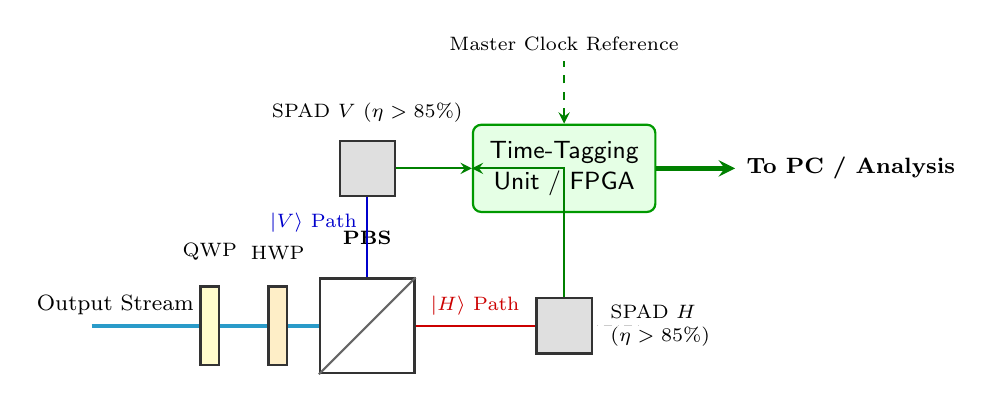
\begin{tikzpicture}[
    >=latex,
    font=\sffamily\small,
    optical/.style={draw=black!80, thick, fill=white},
    beam/.style={draw=cyan!80!black, ultra thick},
    hbeam/.style={draw=red!80!black, thick},
    vbeam/.style={draw=blue!80!black, thick},
    signal/.style={draw=green!50!black, thick, ->, >=stealth},
    spad/.style={rectangle, draw=black!80, fill=gray!25, thick, minimum width=0.7cm, minimum height=0.7cm},
    block/.style={rectangle, draw=blue!80!black, fill=blue!5, thick, rounded corners=3pt, align=center, inner sep=6pt}
]

    % --- Input Axis ---
    \draw[black!20, dash dot] (-1,0) -- (6,0);
    \draw[beam] (-1,0) -- (0.5,0) node[pos=0.2, above, font=\footnotesize] {Output Stream};

    % --- Waveplates (Tomography Stage) ---
    % QWP
    \node[optical, fill=yellow!20, minimum width=0.15cm, minimum height=1.0cm] (qwp) at (0.5,0) {};
    \node[above=0.2cm of qwp, font=\xsfit] {QWP};
    
    % HWP
    \node[optical, fill=yellow!40!orange!20, minimum width=0.15cm, minimum height=1.0cm, right=0.6cm of qwp] (hwp) {};
    \node[above=0.2cm of hwp, font=\xsfit] {HWP};

    \draw[beam] (qwp) -- (hwp);
    \draw[beam] (hwp) -- (2.5,0);

    % --- Polarizing Beam Splitter (PBS) ---
    \node[optical, minimum size=1.2cm] (pbs) at (2.5,0) {};
    \draw[black!60, thick] (pbs.south west) -- (pbs.north east);
    \node[above=0.3cm of pbs, font=\xsfit\bfseries] {PBS};

    % --- Split Paths ---
    % Transmitted (Horizontal - H)
    \draw[hbeam, ->] (pbs.east) -- (5.0,0) node[pos=0.4, above, font=\xsfit\color{red!80!black}] {$|H\rangle$ Path};
    
    % Reflected (Vertical - V)
    \draw[vbeam, ->] (pbs.north) -- (2.5,2.0) node[pos=0.5, left, font=\xsfit\color{blue!80!black}] {$|V\rangle$ Path};

    % --- SPAD Detectors ---
    % SPAD H
    \node[spad] (spadh) at (5.0,0) {};
    \node[right=0.1cm of spadh, font=\xsfit, align=left] {SPAD $H$\\($\eta > 85\%$)};

    % SPAD V
    \node[spad] (spadv) at (2.5,2.0) {};
    \node[above=0.1cm of spadv, font=\xsfit, align=center] {SPAD $V$ ($\eta > 85\%$)};

    % --- Electronic Processing ---
    \node[block, fill=green!10, draw=green!60!black] (tagger) at (5.0,2.0) {Time-Tagging\\Unit / FPGA};

    % Signal Lines to Tagger
    \draw[signal] (spadh.north) |- (tagger.west);
    \draw[signal] (spadv.east) -- (tagger.west);

    % --- Master Clock Reference ---
    \draw[signal, dashed, <-] (tagger.north) -- ++(0,0.8) node[above, font=\xsfit] {Master Clock Reference};

    % --- Final Data Output ---
    \draw[signal, ultra thick] (tagger.east) -- ++(1.0,0) node[right, font=\footnotesize\bfseries] {To PC / Analysis};

\end{tikzpicture}
\caption{Final Polarization Readout \& Tomography Module}
\label{fig:final-detector}

\end{figure}

and using the detectors in the right manner, we're able to figure out which results occur with which probabilities and with which results of the other "qubits", we can find the final states of the system with minimal external computation.

\subsection{Engineering Trade-offs and Limitations}
    \label{sec:Engineering Trade-offs and Limitations}
Considering an AOM of 100 MHz, we can achieve a temporal resolution of 10 ns. This allows for precise control over the timing of the target qubit's passage through the AOM, ensuring that it is either flipped or passed unchanged based on the control qubit's state. The temporal selection mechanism effectively simulates the CNOT operation by leveraging the timing of the control and target beams, and while it does require future CNOTs to use more time to set their probabilities, the nanoscale timing allows the overall computation to still be extremely efficient. The main drawback to this design is the exponential growth factor, where the amount of time required to perform a computation grows exponentially with the number of qubitsand the amount of hardware required to implement such grows at a rate dependent on the algorithm (typically exponentially). However, the amount of time needed starts so low that even up until around 30-40 qubits, the time required is still extremely low (on the order of milliseconds to seconds, even a handful of hours at the high end). Further, the amount of hardware required is still far cheaper than that of a true quantum computer, and the cost of this design is far lower than that of a true quantum computer. 


% ============================================================
%  6. DISCUSSION
% ============================================================
%  7. CONCLUSION
% ============================================================


%  REFERENCES
% ============================================================

    \newpage
    \bibliographystyle{amsplain}     % swap for: apalike, plain, ieee, apa

% ── Inline fallback (no .bib file needed for quick testing) ─
% Comment out the two lines above and uncomment below:
%
% \begin{thebibliography}{9}
%
% \bibitem{AuthorYear}
%   Author, A.\ B., \& Author, C.\ D.\ (Year).
%   Title of the article.
%   \textit{Journal Name}, \textit{Volume}(Issue), pages.
%   \url{https://doi.org/xxxxx}
%
% \end{thebibliography}


\end{document}